\maketitle
\setcounter{page}{1}
\tableofcontents
\newpage
\pagenumbering{arabic}
\section{Theorie}
Ziel des Versuchs ist die Untersuchung der Temperaturabhängigkeit des glühelektrischen
Effektes an einer Hochvakuumdiode. Als glühelektrischen Effekt wird die Emission von Elektronen aus einem
aufgeheizten Metall bezeichnet. Dabei muss an den Elektronen die sogenannte
Austrittsarbeit geleistet werden. Zur Erklärung dieses Begriffs ist die Vorstellung
des Metalls als Potentialtopf sinnvoll. Die positiv geladenen Kerne sind ein einem
Gitter gebunden, das Potential der Kerne erzeugt einen Potentialtopf, der um $\phi$
vom umgebenden Potential abweicht. In diesem
Topf können sich die Elektronen frei bewegen, sie sind nicht mehr an ein Atom gebunden.
Um den Potentialtopf verlassen zu können, müssen die Elektronen mindestens dieses Potential
überwinden. Zusätzlich müssen sie die $\textsc{Fermische}$ Grenzenergie $\zeta$ besitzen,
die aus dem $\textsc{Pauli}$-Prinzip resultiert. Sie entspricht der Energie, die
die Elektronen am absoluten Nullpunkt besitzen würden. Diese Überlegung führt zusammen
mit einigen Kentnissen über das Verhalten der Elektronen in ihrem Phasenraum auf die
$\textsc{Richardson}$-Gleichung
\begin{equation}
  j_S(T) = 4 \pi \frac{e_0 m_0 k^2}{h^3} T^2 \exp\left(\frac{-e_0 \phi}{k T} \right),
  \label{eq:3}
\end{equation}
mit der aus der Temperatur $T$ die Sättigungsstromdichte, also den Strom der Elektronen
aus der Metalloberfläche, berechnet werden.\\
\begin{figure}
  \centering
  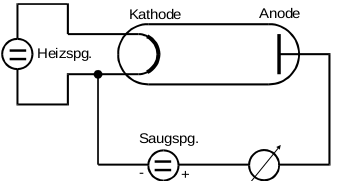
\includegraphics[scale=0.4]{hvdiode.png}
  \caption{Aufbau einer Hochvakuumdiode mit Heizkreislauf\cite{anleitung}.}
  \label{abb:5}
\end{figure}
Versuchsanordnungen zur Messung dieses Zusammenhanges schließen zwangsläufig ein
Vakuum ein, um Wechselwirkungen zwischen emitierten Elektronen und Umgebung zu Verhindern.
Zusätzlich wird in ihnen ein elektrisches Feld angelegt, um die ungerichtete Elektronenemission
zu fokusieren. Dafür wird eine Anode in die Anordnung gebracht, die Emitierende Metaloberfläche
dient als Kathode. Die Elektronen bewegen sich also nach ihrer Emission auf die Anode zu.
Einen solchen Aufbau bezeichnet man als Hochvakuumdiode (siehe Abbildung \ref{abb:5}). Bei Nutzung einer solchen
Anordnung stellt man jedoch fest, dass der an der Anode gemessene Strom von der Spannung
der Anode abhängt und erst ab einer Sättigungsspannung $I_S$ alle Elektronen die Annode erreichen.
Grund dafür ist die Beschleunigung, die die Elektronen im elektrischen Feld erfahren.
Die Ladungsdichte $\rho$ im inneren der Diode ist somit Ortsabhängig. Als Konsequenz der
Kontinuitätsgleichung
\begin{equation}
  j = - \rho v
\end{equation}
wird das elektrische Feld nahe der Kathode sehr schwach, da es von
den austretenden Elektronen abgeschirmt wird. Die nachströmenden Elektronen können
die Anode dann nicht mehr erreichen. Der an der Annode gemessene Strom kann sich
also nur an den Sättigungsstrom annähern. Aus der $\textsc{Poisson}$-Gleichung
und der Energieerhaltung folgt für den Verlauf der Stromdichte in der Diode:
\begin{equation}
  j = \frac{4}{9} \varepsilon_0 \sqrt{2 e_0 / m_0} \frac{a^2}{V^{3/2}},
  \label{eq:4}
\end{equation}
das sogenannte $\textsc{Langmuir-Schottkysche}$ Raumladungsgesetz. $a$ bezeichnet dabei
die $x$-Position der Anode.\\
Aus \eqref{eq:4} folgt, dass ohne anliegendes Potential ($V \le 0$) kein Anodenstrom messbar ist.
In der Realität lässt sich aufgrund der Geschwindigkeit, die die Elektronen auch ohne
anliegende Spannung besitzen, ein gewisser Strom messen. Dieser Strom wird Anlaufstrom
genannt. Die Energie der Elektronen muss jedoch auch groß genug sein, ein äußeres
Potential $V$ zu überwinden. Allgemein erhält man für die Anlaufstomstärke:
\begin{equation}
  j(V) = j_0 \exp\left(-\frac{e_0 \phi_A + e_0 V}{kT}\right),
  \label{eq:5}
\end{equation}
wobei $\phi_A$ die Austrittsarbeit des Anodenmaterials bezeichnet, die ebenfalls
überwunden werden muss.\\
Die Kombination der durch \eqref{eq:5}, \eqref{eq:4} und \eqref{eq:3} beschriebenen Abhängigkeiten
liefern die sogenannte Kennlinie der Hochvakuumdiode. Ohne anliegende Spannung kann nur
ein Anlaufstrom gemessen werden. Wird die Spannung erhöht, misst man die $V^{3/2}$-Abhängigkeit
des Raumladungsgesetzes. Steigt die Spannung weiter, so strebt der gemessene Anodenstrom gegen
einen Sättigungswert. Ein Beispiel für eine Kennline bei konstantem $T$ ist in \ref{abb:6}
gegeben.
\begin{figure}
  \centering
  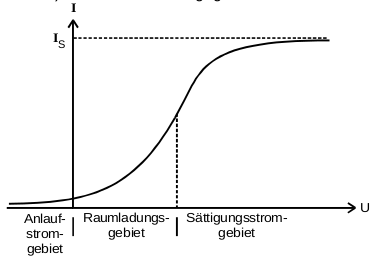
\includegraphics[scale=0.4]{kennlinie.png}
  \caption{Beispielhafte Kennline mit Kennzeichnung der einzelnen Abschnitte\cite{anleitung}.}
  \label{abb:6}
\end{figure}
\section{Durchführung}
\subsection{Versuchsaufbau}
Zur Aufnahme von Kennlinien wird ein XY-Schreiber über Widerstände in die Verbindung zwischen
Kathode und Annode und Kathode eingebunden. In diesem Kreislauf ist zur Erzeugung
des Potentials ein regelbares Konstantspannungsgerät eingebunden. Die in diesem
Kreislauf anliegenden Spannungen und Stromstärken werden über Messgeräte gemessen.
In einem zweiten Kreislauf wird an der Kathode ein Konstantspannungsgerät zur Erzeugung
der Heizspannung angeschlossen. Auch hier wird die Spannung gemessen (siehe \ref{abb:7}).
Für die Messung der Anlaufstromkurve wird eine abgewandelte Version dieser Schaltung
verwendet. Der XY-Schreiber wird entfernt, ebenso das Spannungsmessgerät des Annode-Kathode
Kreislaufs. Das Amperemeter wird durch eines mit Messbereich im \si{\nano\ampere}
Bereich ersetzt (siehe \ref{abb:8}).
\begin{figure}
\centering
  \begin{subfigure}{0.4\textwidth}
    \centering
    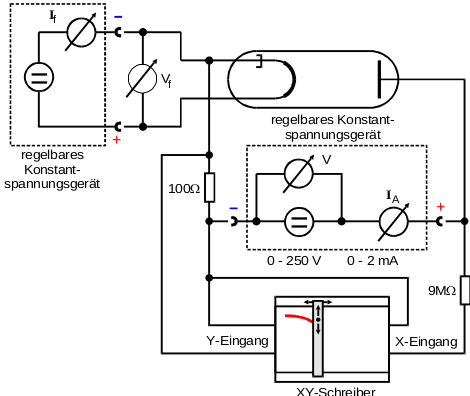
\includegraphics[width=\textwidth]{aufbkenn.png}
    \caption{Versuchsaufbei zur Bestimung von Kennlinen\cite{anleitung}.}
    \label{abb:7}
  \end{subfigure}
  \begin{subfigure}{0.4\textwidth}
    \centering
    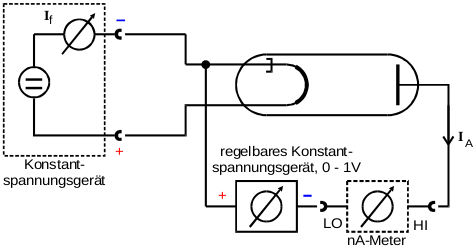
\includegraphics[width=\textwidth]{aufbanl.png}
    \caption{Versuchaufbau zur Bestimmung des Anlaufstroms\cite{anleitung}.}
    \label{abb:8}
  \end{subfigure}
  \caption{Übersicht über die Versuchsaufbauten.}
\end{figure}
\subsection{Versuchsdurchführung}
In einem ersten Versuchsteil wird die Temperaturabhängigkeit des Sättigungsstroms ermittelt.
Dazu werden für verschiedene Heizspannungen jeweils eine Kennline aufgenommen.
Die erzeugte Temperatur wird jewils aus der Leistungsbilanz des Heizkreislaufs bestimmt.
Daraus wird dann die Austrittsarbeit der Kathode bestimmt.
In einem folgenden Versuchsteil wird für die maximale Heizspannung
aus einer Kennline der Gültigkeitsbereich von \eqref{eq:4} ermittelt und der
Tatsächlie Exponent der $V$-Abhängigkeit bestimmt. Desweiteren wird der Anlaufstrom
gemessen und daraus $T$ bestimmt.

\section{Auswertung}
\section{Diskussion}
\newpage
\nocite{*}
\printbibliography
